% vim:spell:spelllang=en

\tikzstyle cfgnodewl=[circle, draw=black, fill=white, inner sep=1pt, minimum width=4pt]
\tikzstyle cfgnode=[rectangle,draw,inner sep=4pt, minimum width=1.6cm,minimum height=12pt]
\tikzstyle cfgedge=[-stealth]
\tikzstyle cfgpath=[style=cfgedge, snake=snake, segment amplitude=.4mm, segment length=2mm, line after snake=1mm]
\tikzstyle cfgbe=[style=cfgedge, dashed]

\newcommand{\exgraph}[4]{
	\draw (0,3.7)     node[cfgnode] (l1) { #1 };
	\draw (1.0,1.8)   node[cfgnode] (l2) { #2 };
	\draw (-1.0,1.8)  node[cfgnode] (l3) { #3 };
	\draw (0,-0.1)    node[cfgnode] (l4) { #4 };
	\draw[cfgedge] (l1) -- (l2);
	\draw[cfgedge] (l1) -- (l3);
	\draw[cfgedge] (l2) -- (l4);
	\draw[cfgedge] (l3) -- (l4);
}

\newcommand{\loopedgeR}[2]{([xshift=3mm] #1.south) |- ([shift={(3mm, -3mm)}] #1.south east) -- ([shift={(3mm, 3mm)}] #2.north east) -| ([xshift=3mm] #2.north)}
\newcommand{\loopedgeRM}[3]{([xshift=3mm] #1.south) |- ([shift={(3mm, -3mm)}] #1.south east) -- (#2) -- ([shift={(3mm, 3mm)}] #3.north east) -| ([xshift=3mm] #3.north)}
\newcommand{\loopedgeL}[2]{([xshift=-3mm] #1.south) |- ([shift={(-3mm, -3mm)}] #1.south west) -- ([shift={(-3mm, 3mm)}] #2.north west) -| ([xshift=-3mm] #2.north)}

\newcommand{\insnlist}[3]{
\begin{array}{rcl}
#1 & \gets  & #2 \\
   & \vdots & \\
#3 & \gets  & #1 \\
   & \gets  & #3 \\
\end{array}
}


\newcommand{\iuse}[1]{\gets\var #1}
\newcommand{\idef}[1]{\var #1\gets}
\newcommand{\var}[1]{\mathtt{#1}}
\newcommand{\phiop}{$\phi$-function}
\newcommand{\phiops}{\phiop s}
\newcommand{\dom}{\preceq}
\newcommand{\sdom}{\prec}
\newcommand{\phizero}{\ensuremath{\phi_0}}

% \newcommand{\domzone}[1]{\mathit{dom}({#1})}
% \newcommand{\sdomzone}[1]{\mathit{sdom}({#1})}
% \newcommand{\ldef}[1]{#1}
% \newcommand{\luse}[1]{\mathit{uses}\,#1}
% \newcommand{\DF}[1]{\mathrm{DF}_{#1}}
% \newcommand{\IDF}{\mathrm{DF}^+}
% \newcommand{\JS}[1]{\mathcal{J}_{#1}}
% \newcommand{\IJS}{\JS{\infty}}
% \newcommand{\nepath}[2]{{#1}{\overset{+}{\rightarrow}}{#2}}

\title{SSA Reconstruction}
\author{Sebastian Hack}

\chapter{SSA Reconstruction \Author{S. Hack}}
% \numberofpages{6}

\section{Introduction}

Some optimizations break the single-assignment property of the SSA form by inserting additional definitions for a single SSA value.
A common example is live-range splitting by inserting copy operations or inserting spill and reload code during register allocation.
Other optimizations, such as loop unrolling or jump threading, perform similar operations.
Let us first go through two examples before we present algorithms to repair SSA.

\subsection{Live-Range Splitting}

In Figure~\ref{fig:nonssa}, our spilling pass decided to spill a part of the live range of the variable~$x_0$ in the right block.
Therefore, it inserted a store and a load instruction. 
The load however is a second definition of $x_0$, hence SSA is violated and has to be reconstructed as shown in Figure~\ref{fig:recons}.

\begin{figure}[htbp]
	\centering
	\subfigure[Original program] {
		\label{fig:harmless}
		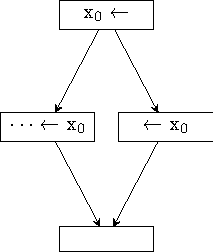
\includegraphics[width=0.3\textwidth]{spill_orig.pdf}
		% \input spill_orig.tikz
	}
	\hfill
	\subfigure[Spilling~$x_0$, SSA violated] {
		\label{fig:nonssa}
		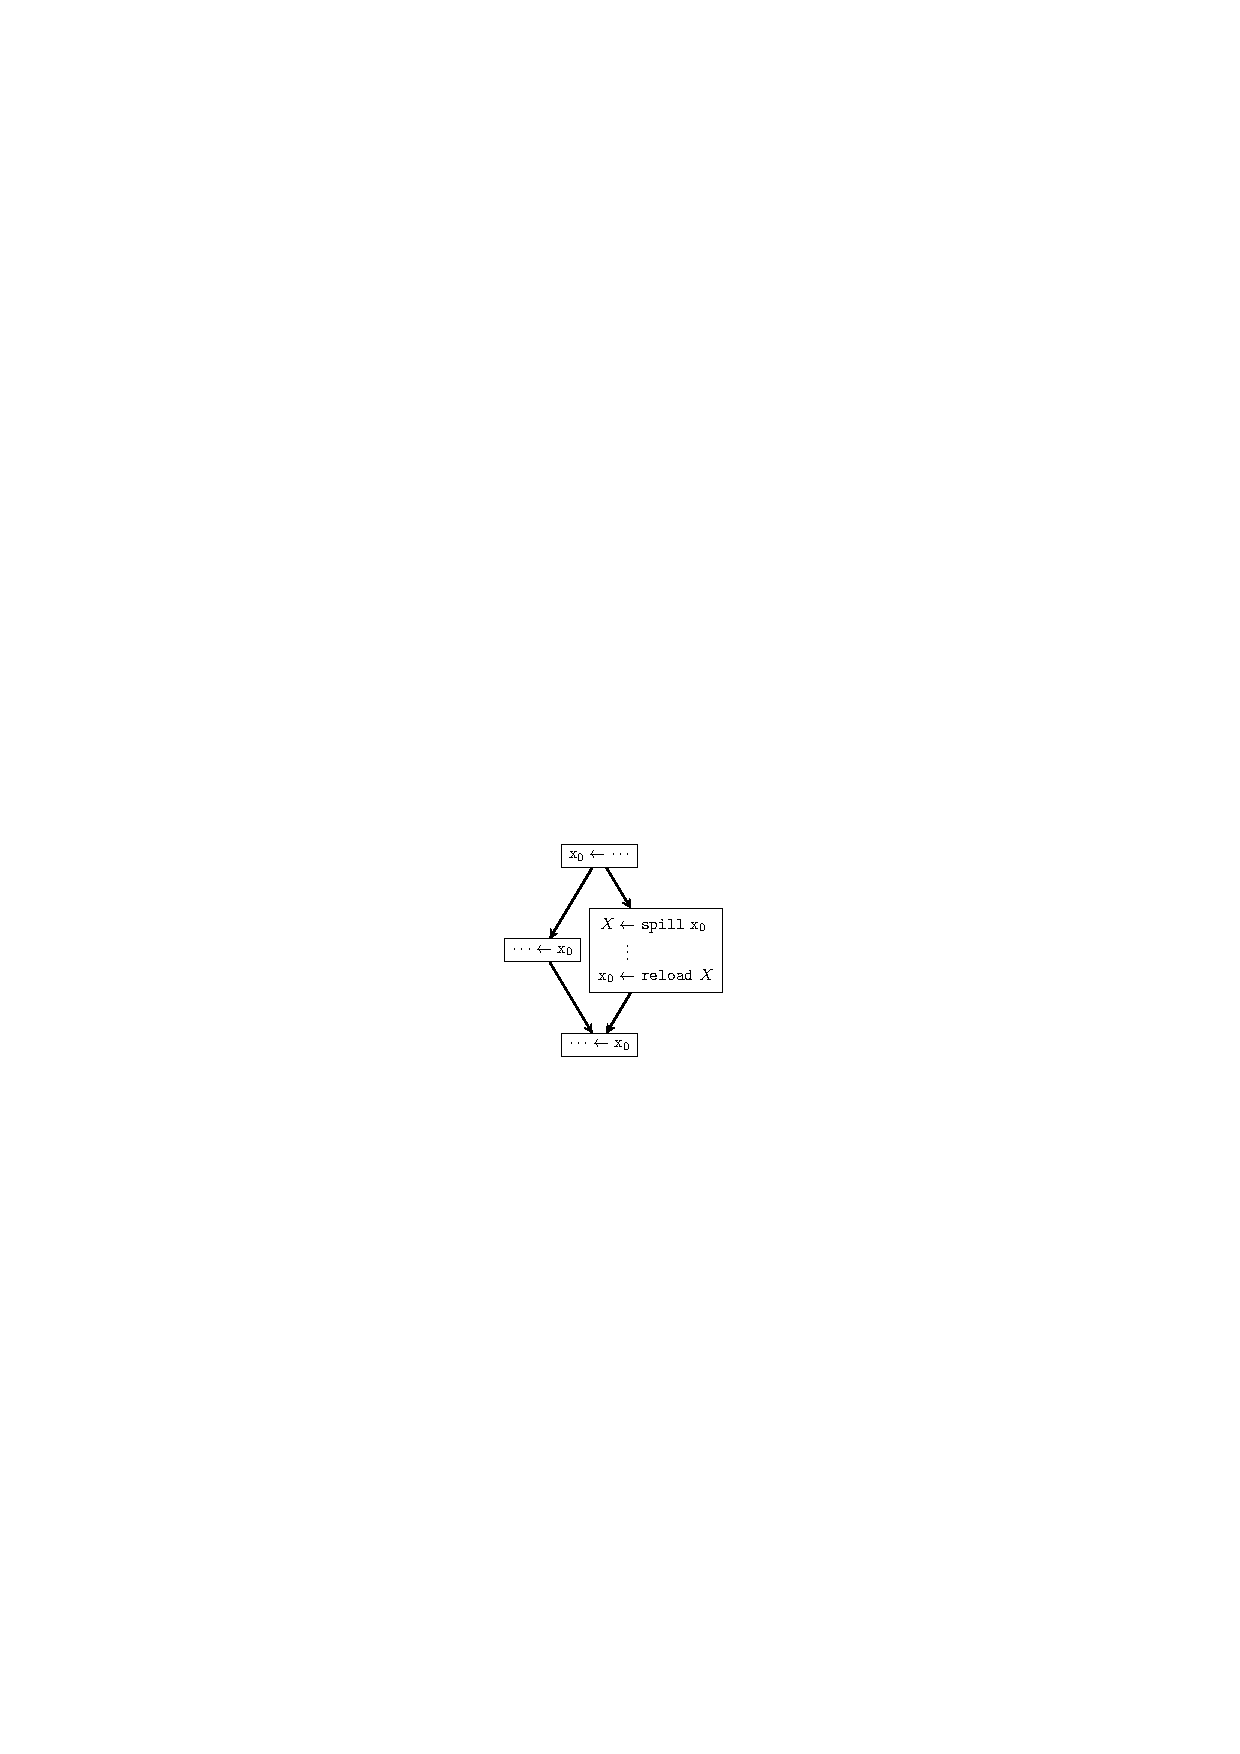
\includegraphics[width=0.3\textwidth]{spill_nonssa.pdf}
	}
	\hfill
	\subfigure[SSA reconstructed] {
		\label{fig:recons}
		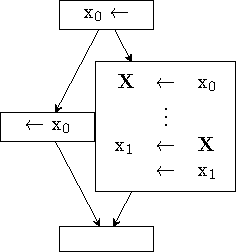
\includegraphics[width=0.3\textwidth]{spill_recons.pdf}
	}
	\label{fig:ex1}
	\caption{Adding a second definition}
\end{figure}

In a more complicated configuration, adding a second definition to an SSA variable can cause \phiops\ to be inserted.
Figure~\ref{fig:withphis} shows the same program fragment with the left use of~$\var x_0$ being moved to the bottom.
As there are two definitions reaching the use in the lower block, a \phiop\ has to be inserted. 

\begin{figure}[htbp]
	\centering
	\subfigure[Original program] {
		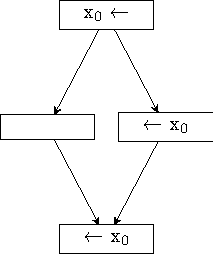
\includegraphics[width=0.3\textwidth]{spill_phi_orig.pdf}
	}
	\qquad
	\subfigure[Second definition of~$\var x_0$, \phiop\ inserted] {
		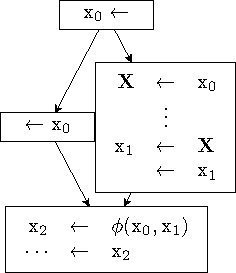
\includegraphics[width=0.3\textwidth]{spill_phi.pdf}
	}
	\caption{SSA repaired}
	\label{fig:withphis}
\end{figure}

Such program modifications are done by many optimizations. 
Not surprisingly, maintaining SSA is often one of the more complicated and error-prone parts in such optimizations;
owing to the insertion of additional \phiops\ and the correct redirection of the variable's uses.

\subsection{Loop Unrolling}

Loop unrolling is a transformation to increase instruction-level parallelism inside the body of a loop.
To this end, the body of the loop is duplicated $n$~times. 
Similar to the example above, this adds several new definitions \emph{and} uses to an existing SSA variable. 
Consider following example and assume that the loop's body is duplicated once, i.e.~the loop is unrolled once.

\begin{figure}[htbp]
	\begin{center}
		\subfigure[Original loop] {
			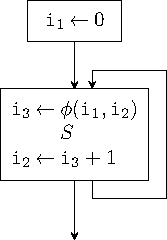
\includegraphics[width=0.3\textwidth]{loop_orig.pdf}
		}
		\hfill
		\subfigure[Unrolled loop, code duplicated, SSA broken] {
			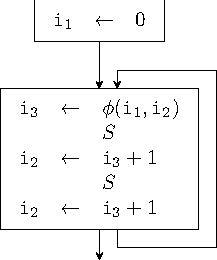
\includegraphics[width=0.3\textwidth]{loop_unroll.pdf}
		}
		\hfill
		\subfigure[SSA repaired] {
			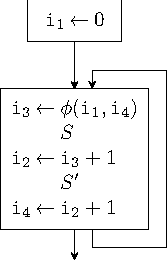
\includegraphics[width=0.3\textwidth]{loop_unroll_repair.pdf}
		}
	\end{center}
	\caption{Loop Unrolling}
	\label{fig:unroll}
\end{figure}

These examples show that naive code duplication and live-range splitting in an SSA program can violate the single assignment property of the SSA form.
To repair these effects, we seek for a simple, black box like algorithm.
Ideally, we provide a set of definitions and uses of which we claim that they correspond to one single non-SSA variable.
Afterwards, the algorithm establishes the SSA form for these live ranges.
This includes re-assigning the uses to the correct definition and inserting \phiops\ on demand.
Next, we investigate an algorithm based on the classical dominance frontier construction algorithm.

\section{General Considerations}
We consider following scenario:
The program is represented as a control-flow graph (CFG) and is in SSA form.
For the sake of simplicity, we assume that each instruction in the program only writes to a single variable.
Due to the single-assignment property of the SSA form, we can then identify the program point of the instruction and the variable. 
An optimization/transformation now violates SSA by inserting additional definitions for an existing SSA variable, like in the examples above.
The original variable and the additional definitions can be seen as a single non-SSA variable that has multiple definitions and uses.

In the following, $v$ will be a such a non-SSA variable.
$D$~is a set of SSA variables being the definitions of~$v$.
A use of a variable is a pair consisting of a program point (a variable) and an integer denoting the index of the operand at the using instruction.

Both algorithms which we are going to present share the same driver routine (Figure~\ref{alg:ssaconstr_driver}).
First, every basic block~\verb|b| is equipped with a list~\verb|b.defs| that contains all instructions in the block which define one of the variables in~$D$.
This list is sorted according to the schedule of the instructions in the block from back to front.
Hence, the latest definition is the first in the list.

Then, all uses of the variables in~$D$ are scanned.
We search the use's block for a definition of the used variable.
By scanning the block's list from back to front, we find the latest such use if one exists. 
If the variable has no definition in the block, we have to find the definition that reaches this block from \emph{outside.}
Here we have to differentiate of the user is a \phiop{} or not.
If it is a \phiop{} the block of the use the corresponding predecessor block.
We use two functions \verb|find_def_from_begin| and \verb|find_def_from_end| that find the reaching definition at the beginning and end of a block, respectively. 
As can seen from Algorithm~\ref{alg:ssaconstr_driver}, \verb|find_def_from_end| can be expressed in terms of \verb|find_def_from_begin|. 
The only difference is that \verb|find_def_from_end| considers definitions in the block. 
Our two approaches only differ in the implementation of the function \verb|find_def_from_begin|.
The differences are described in the next two sections.
\begin{algorithm}
	\caption{SSA Reconstruction Driver}
	\label{alg:ssaconstr_driver}

\begin{verbatim}
proc ssa_reconstruct(set of var D):
  for d in D:
    b = d.block
    insert d in b.defs according to schedule
    # latest definition is first in list

  for each use u of D:
    v = get_used_var(u)
    b = v.block
    d = None

    # search for a local definition in the block
    for e in b.defs:
      if v == e and is_later(u, e):
        d = e
        break
        
    # no local definition was found, search in the predecessors
    if d == None:
      # if the user is a phi we have to start the search 
      # at the end the corresponding predecessor block 
      if u.is_phi():
        d = find_def_from_end(u.block.pred(u.index), ...)
      else:
        d = find_def_from_begin(b, ...)

    rewrite use at u to d

proc find_def_from_end(block b, ...):
  if not b.defs.empty():
    return b.defs[0]
  return find_def_from_begin(b, ...)
\end{verbatim}
\end{algorithm}

\section{Reconstruction based on the Dominance Frontier}
This algorithm follows the same principles as the classical SSA construction algorithm by Cytron et al.~\cite{cytron:1991:ssa}.
We compute the iterated dominance frontier (IDF) of $D$ (cf.~Appel's book~\cite{appel:2002:modern} for an algorithm on how to compute the IDF).
This set is a sound overapproximation on the set where \phiops{} must be placed (it might contain blocks where a \phiop{} would be dead).
Then, we search for each use the corresponding reaching definition.
This search starts at the block of~$u$.
If that block is in the IDF of~$D$ a \phiop{} needs to be placed at its entrance.
The operands of that \phiop{} are then (recursively) searched in the predecessors of the block.
If the block is not in the IDF, the search continues in the block's immediate dominator. 
This is because in SSA every use of a variable must be dominated by its definition\footnote{The definition of an operand of a \phiop{} has to dominate the according predecessor block.}.
If the block is not in the IDF, the reaching definition is the same for all predecessors and hence for the immediate dominator of this block.
Note that by re-wiring the usages of several variables, some variables defined by \phiops\ may not be used anymore.
A dead code elimination pass after SSA reconstruction will remove these. 
Algorithm~\ref{alg:ssaconstr} shows this procedure in pseudo-code.

\begin{algorithm}
  \caption{SSA Reconstruction based on Dominance Frontiers}
  \label{alg:ssaconstr}
\begin{verbatim}
proc find_def_from_begin(block b, set of blocks F):
  if b in F:
    d = new_phi(b)
    i = 0
    for p in b.preds: 
      o = find_def_from_end(p, F)
      set i-th operand of d to o
      i = i + 1
  else:
    d = find_def_from_end(b.idom, F)
  b.def = d
  return d
\end{verbatim}
\end{algorithm}

\section{Search-based Reconstruction}

The second algorithm we present here is similar to the construction algorithm that Click describes in his thesis~\cite{click:thesis}.
Although his algorithm is designed to construct SSA from the abstract syntax tree, it also works well on control flow graphs.
Its major advantage over the algorithm presented in the last section is that it does neither require dominance information nor dominance frontiers.
Thus it is well suited to be used in transformations that change the control flow graph.
Its disadvantage is that potentially more blocks have to visited during the reconstruction.
The principle idea is to start a search from every use to find the corresponding definition inserting \phiops\ on the fly while caching the found definitions at the basic blocks.
This is similar to the implementation of a data-flow analysis, that places the \phiops.
As in the last chapter, we only consider the reconstruction for a single variable.
If multiple variables have to be reconstructed, the algorithm can be applied to each variable separately.

We perform a backward depth-first search in the CFG to collect the reaching definitions at each block. 
To mark a block as visited, the reaching definition of that block is inserted into the \verb|defs| list of that block.
If the CFG is a DAG, all predecessors of a block can be visited before the block itself is processed (post-order traversal).
Hence, all reaching definitions at a block~\verb|b| can be computed before we decide whether to place a \phiop{} in~\verb|b| or not.
If more than one definition reaches the block, we need to place a \phiop.

If the CFG has loops, there are blocks for which not all reaching definitions can be computed before we can decide whether a \phiop{} has to be placed.
Recursively computing the reaching definitions for a block~\verb|b| can end up at~\verb|b| itself.
To avoid infinite recursion, we create a \phiop{} without operands in the block before descending to the predecessors. 
Hence, if a variable has no definition in a loop, the \phiop{} placed in the header eventually reaches itself (and can later be eliminated). 
When we return to~\verb|b| we decide whether a \phiop{} has to be placed in~\verb|b| by looking at the reaching definition for every predecessor.
If the set of reaching definitions is a subset of $\{a,x\}$ where~$x$ is the \phiop{} inserted at~\verb|b|, then no \phiop{} is necessary and we can propagate~$a$ further downwards. 
Otherwise, we place a \phiop.

\begin{algorithm}
	\caption{Search-based SSA Reconstruction}
	\label{alg:ssaconstr_click}

\begin{verbatim}
proc find_def_from_begin(block b):
  phi = make_phi()
  if b.defs.empty():
    b.defs = [ phi ] 

  reaching_defs = []
  for p in b.preds:
    reaching_defs += find_def_from_end(p)
  if phi_necessary(reaching_defs):
    set_arguments(phi, reaching_defs)
    d = phi
  else:
    reaching_defs.remove(phi)
    d = reaching_defs[0]
  return d
\end{verbatim}
\end{algorithm}

\section{Conclusions}

Some optimizations, such as loop unrolling or live-range splitting destroy the single-assignment property of the SSA form.
In this chapter we presented two generic algorithms to reconstruct SSA.
The algorithms are independent of the transformation that violated SSA and can be used as a black box:
For every variable for which SSA was violated, a routine is called that restores SSA.
The presented algorithms differ in the prerequisites and their runtime behavior:
\begin{enumerate}
	\item 
		The first is based on the iterated dominance frontiers like the classical SSA construction algorithm by Cytron et al.~\cite{cytron:1991:ssa}.
		Hence, it is less suited for optimizations that also change the flow of control since that would require recomputing the iterated dominance frontiers.
		On the other hand, by using the iterated dominance frontiers, the algorithm can find the reaching definitions quickly by scanning the dominance tree upwards.
	\item 
		The second algorithm does not depend on additional analysis information such as iterated dominance frontiers or the dominance tree.
		Thus, it is well suited for transformations that change the CFG because no information needs to be recomputed.
		On the other hand, it might find the reaching definitions slower than the first one because they are searched by a depth-first search in the CFG.
\end{enumerate}
Both approaches constructed \emph{pruned} SSA (TODO: cite other chapter), i.e.~no \phiop{} is dead. 
One can also show that the first approach produces minimal SSA in the sense of Cytron et al.~\cite{cytron:1991:ssa} whereas the second approach might create superfluous \phiops{} in the case of irregular control flow.
